\documentclass{article}
\setlength{\parskip}{5pt} % esp. entre parrafos
\setlength{\parindent}{0pt} % esp. al inicio de un parrafo
\usepackage{amsmath} % mates
\usepackage[sort&compress,numbers]{natbib} % referencias
\usepackage{url} % que las URLs se vean lindos
\usepackage[top=25mm,left=20mm,right=20mm,bottom=25mm]{geometry} % margenes
\usepackage{hyperref} % ligas de URLs
\usepackage{graphicx} % poner figuras
\usepackage[spanish]{babel} % otros idiomas
\usepackage[utf8]{inputenc}
\author{Alfredo Cárdenas Mena \\
Daniel Garcia Rodarte\\
Angel Eduardo Gonzalez Melendres \\
Angel Mario Alcala Rodriguez \\
Aarón Lozano Aguilar} % author
\title{Actividad 2: Prótesis de Mano} % titulo
\date{\today}
\usepackage{float} 
\begin{document} % inicia contenido

\maketitle % cabecera
\begin{abstract} % resumen
Las prótesis en las manos, son muy importantes hoy en día, ya que les ayuda en dado caso que haya una ausencia de la mano, cada año la tecnología nos ayuda poder actualizar las prótesis, para poder así que esta sea más fácil de manejarla, todo esto conlleva en muchos procesos, como lo son los mecanismos y el estudio de como nuestro cuerpo y cerebro responden a cada una de ellas. 
\end{abstract}

\section{Introducción}\label{intro} % seccion y etiqueta

 
Una protesis es una sustitución de una parte del esqueleto o de un órgano por una pieza o implante especial, que reproduce más o menos exactamente lo que ha de sustituir. También se denomina de este modo a la pieza o implante artificial implantado en el organismo. Los avances en el diseño de prótesis están directamente relacionados con los avances en el procesamiento de los materiales utilizados por los humanos, así como con el desarrollo de la tecnología y la comprensión de la biomecánica humana. Las prótesis son artículos diseñados para mejorar o reemplazar un miembro funcional, parcial o total del cuerpo humano afectado, por lo que la prótesis para amputados también trabaja con el desarrollo psicológico del amputado, creando una sensación de plenitud, restaurando la movilidad y la apariencia.
\\
El nivel de amputación o el tipo de displasia que requiere tratamiento juega un papel importante en la selección de una prótesis adecuada. En base a los requerimientos de cada paciente, determinar el tipo de dispositivo que mejor se adapte a sus características. (Figura 1). 

\begin{figure}[H] % figura
    \centering
    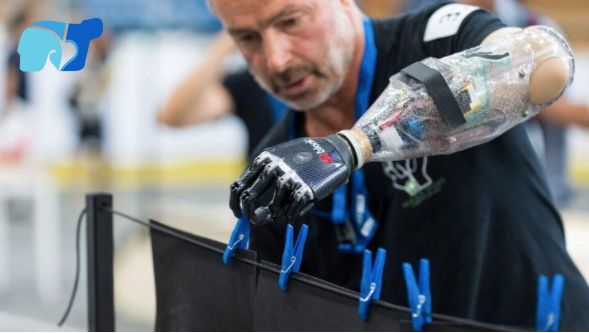
\includegraphics[width=100mm]{EQP 3/Protesis de mano/mano2.jpg}
    \caption{Clasificaciones de prótesis\cite{EvoProte}}
    \label{grafica}
\end{figure}


\section{Desarrollo}
Las prótesis son uno de esos inventos que engrandecen a los humanos como sociedad. Son dispositivos robóticos creados para mejorar la calidad de vida de las personas con amputaciones. De hecho, la prótesis de mano es el dispositivo para amputados con mayor demanda y de mayor complejidad. Las prótesis de mano mecánicas son dispositivos que se usan con la función de cierre o apertura de la mano a voluntad, su control es por medio de un arnés que se encuentra sujeto alrededor de los hombros, parte del pecho y del brazo. Su sistema de agarre es para objetos relativamente grandes y redondos debido a la poca precisión del mecanismo, este tipo de destreza es parte de la pinza gruesa para manipular objetos. Las funciones principales de la mano son la prensión y el tacto. La prensión por si sola se puede conseguir relativamente fácil en una prótesis. Por el contrario, desarrollar una prótesis que sienta es un trabajo especializado de ingeniería, medicina y neurociencia.

\subsection{PRÓTESIS MECÁNICA DE MANO}
Las prótesis de mano mecánicas son dispositivos que se usan con la función de cierre o apertura de la mano a voluntad, su control es por medio de un arnés que se encuentra sujeto alrededor de los hombros, parte del pecho y del brazo. Su sistema de agarre es para objetos relativamente grandes y redondos debido a la poca precisión del mecanismo, este tipo de destreza es parte de la pinza gruesa para manipular objetos.


\begin{figure}[H] % figura
    \centering
    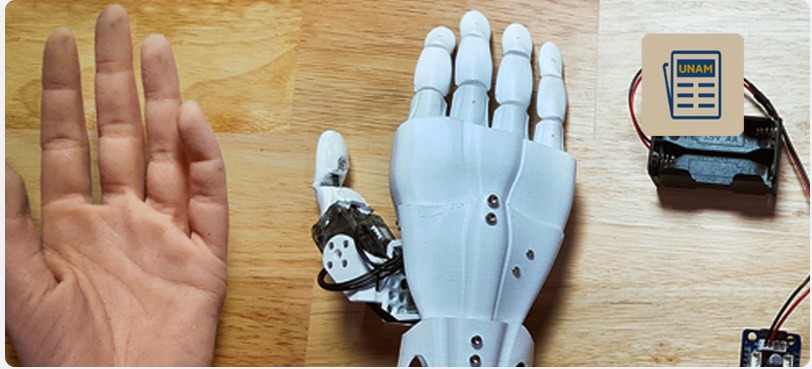
\includegraphics[width=100mm]{protemano.jpeg} % archivo
    \caption{Anatomía de la mano\cite{SisID}.}
    \label{grafica:dos}
\end{figure}

\subsection{PRÓTESIS ELÉCTRICA DE MANO}
Su sistema de función es a partir de motores eléctricos en los dispositivos terminales, muñeca y codo, con una batería recargable. Es posible controlarlas de varias formas: servo control, un botón pulsador o un interruptor con arnés. El precio de adquisición es elevado debido a su mecanismo de función. Existen algunas características a considerar: el mantenimiento es complejo, la baja resistencia a medios húmedos y el peso que puede levantar es mínimo.
\begin{figure}[H] % figura
    \centering
    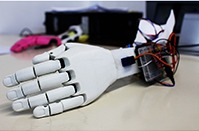
\includegraphics[width=80mm]{EQP 3/Protesis de mano/elemano.jpeg}% archivo
    \caption{Protesis electrica\cite{DiseCons}.}
    \label{grafica:dos}
\end{figure}


\subsection{PRÓTESIS NEUMÁTICAS DE MANO}
Su función depende de ácido carbónico comprimido, que proporciona una gran cantidad de energía. Aunque, presenta como inconveniente las complicaciones de sus aparatos y accesorios, y el riesgo en el uso del ácido carbónico. Su desarrollo fue interrumpido debido a las dificultades técnicas presentadas.
\begin{figure}[H] % figura
    \centering
    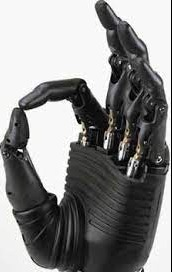
\includegraphics[width=45mm]{EQP 3/Protesis de mano/neuma.jpeg}% archivo
    \caption{Protesis neumaticas\cite{DiseCons}.}
    \label{grafica:dos}
\end{figure}





\subsection{PRÓTESIS HÍBRIDA DE MANO}
Es la combinación con la acción del cuerpo y el accionamiento por electricidad. Este concepto es ampliamente utilizado en las prótesis transhumerales (amputación por encima del codo), donde por lo general el codo es accionado por el cuerpo y el dispositivo terminal (gancho o mano) es de accionamiento mioeléctrico  (Loaiza y Arzola, 2011)
\begin{figure}[H] % figura
    \centering
    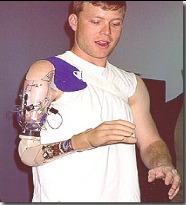
\includegraphics[width=65mm]{EQP 3/Protesis de mano/hibri.jpeg}% archivo
    \caption{Protesis hibrida\cite{AnSe}.}
    \label{grafica:dos}
\end{figure}





\subsection{PRÓTESIS CON ACTUACIÓN HÍBRIDA}
Las prótesis con actuación híbrida, estas manos robóticas combinan la electricidad con la acción del cuerpo. De esta rama se crean las conocidas prótesis de mano mioeléctricas. Las prótesis de mano robóticas basan su funcionamiento en las señales eléctricas de los músculos. Estas señales son conocidas como señales electromiográficas (EMG). Dichas señales se pueden captar cuando se produce la contracción o relajación de un músculo. Las prótesis mioeléctricas tienen una mejor precisión en cuanto al agarre de objetos y la naturalidad del movimiento. Asimismo, su mayor ventaja es que funcionan con la intención de movimiento del paciente. Basta con pensar en querer agarrar un objeto para que nuestro cerebro envíe la señal a la prótesis.

\section{Conclusiones}
El avance medico junto el tecnologico nos han llevado a este tipo de culminaciones biomecanicas, anteriormente era muy difícil tener una y aparte el cómo adaptarse a esta, ya que se tenía que cumplir con ciertos requisitos para ser uno de los seleccionados, la tecnología que se maneja hoy en día, nos ayuda a que sea más fácil el poder contar con una, en este tema se aprendió el cómo estas funcionan y los mecanismos que se utilizan para que tengan  un mejor manejo, un factor importante en este es las simulaciones, ya que este nos ayuda a comprobar que las prótesis estén bien diseñadas, ya que ahí es donde podemos llegar a detectar un error (si en dado caso se llagara a presentar).
Gracias a estos dispositivos tenemos la oportunidad de entrar en estudios investigativos que no tenian antes los ingenieros, simulaciones mecánicas y ahora empezar a conocer la anatomía de la mano saber que hay muchos tipos de prótesis, hace unos años conocí a un ingeniero en mecatrónica que estaba especializado en biodispositivos y tenía prototipos de prótesis para las venas del corazón eran unas prótesis tan chiquitas que quede asombrada de como el hombre puede crear infinidad de cosas para adaptarse a la vida diaria.

\section{Referencias}

\bibliography{refemano.bib}
\bibliographystyle{apacite}


\end{document}